\section{实验八:Locks}\label{sec:Locks}

\subsection{实验目的}

\begin{enumerate}
	\item 理解锁竞争,包括锁竞争产生的原因以及解决方法。
	\item 理解通过增加锁的数量来降低锁竞争的原理,并应用到程序中。
	\item 加深对于使用锁来达到进程互斥方法的掌握程度。 
\end{enumerate}

\subsection{实验内容}

\begin{enumerate}
	\item 重新设计系统管理内存的方式,实现每个 CPU 管理一个空闲链表和一个锁。
	\item 修改系统的 IO 缓冲区,通过散列的方式完成对缓冲区和锁的分割。 
\end{enumerate}

\subsection{实验准备}

阅读 xv6 参考书的第 6 章、第 3.5 节、第 8.1 至 8.3 节。

\subsubsection{竞态条件}

竞态条件是指多个进程读写某些共享数据时,至少有一个访问是写入的情况。

当多个进程在不同 CPU 上并发执行时,如果它们访问共享的数据结构(如内存分配器的空闲链表),就会出现问题。例如,在链表的push操作中,如果两个CPU同时执行,它们可能都在执行 \texttt{l->next = list} 之后,第设置 \texttt{list = l} 之前,这会导致第二次赋值覆盖第一次赋值,造成数据丢失。

锁通过确保互斥访问来避免竞态条件。在临界区域(\texttt{acquire} 和 \texttt{release} 之间的代码)中,同一时间只有一个CPU可以执行,这使得上述的竞态情况不可能发生。锁实际上是将并发的临界区域串行化,确保数据结构的完整性。锁不仅保护数据,更重要的是保护数据结构的不变量。

\begin{figure}[!htb]
	\centering
	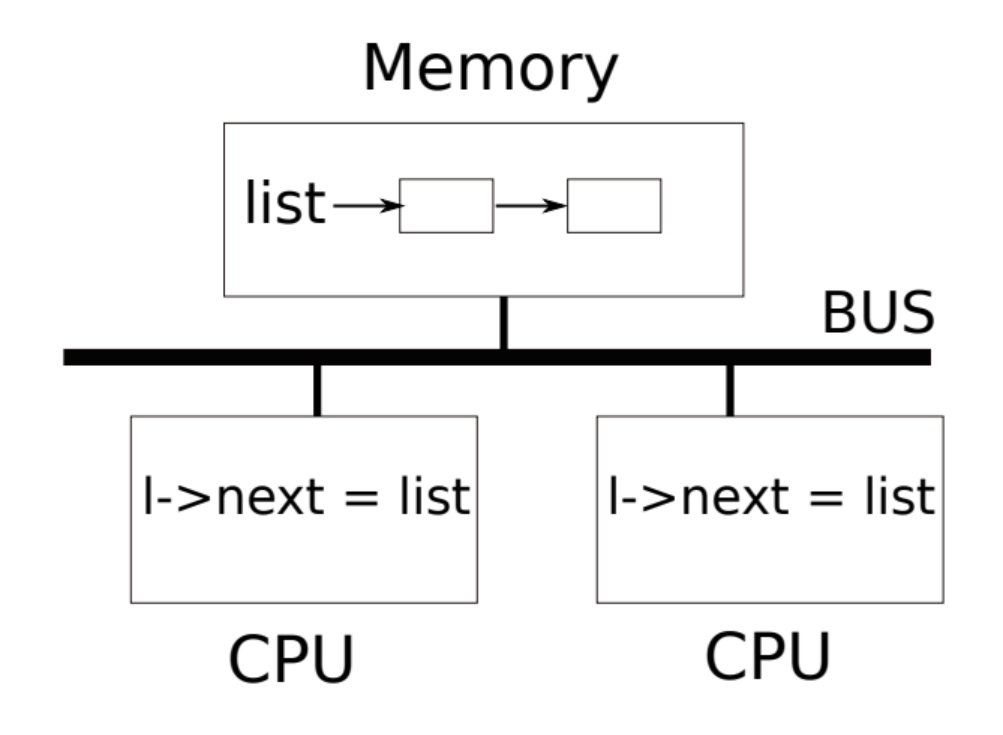
\includegraphics[width=0.4\textwidth]{simplified_SMP}
	\caption{链表位于两个 CPU 的共享内存中}
	\label{fig:simplified_SMP}
\end{figure}

\subsubsection{自旋锁}

Xv6 使用 \texttt{struct spinlock} 来表示自旋锁,其中最重要的字段是 \texttt{locked},当锁可用时为零,当它被持有时为非零。从逻辑上讲,获取锁应该通过检查 \texttt{locked} 字段是否为零,如果是则设置为 1 来获得锁。

简单的锁实现(如检查 \texttt{lk->locked == 0} 然后设置 \texttt{lk->locked = 1})在多处理器环境下无法保证互斥。两个 CPU 可能同时到达检查点,都看到 \texttt{lk->locked} 为零,然后都执行设置操作,导致两个不同的 CPU 持有锁,违反了互斥属性。

为了解决上述问题,需要将检查锁状态和设置锁状态作为原子(不可分割)步骤执行。多核处理器通常提供专门的指令来实现这种原子操作,在 RISC-V 上这条指令是 \texttt{amoswap r, a}。该指令原子地读取内存地址 a 处的值,将寄存器 r 的内容写入该地址,并将其读取的值放入 r 中。它使用特殊的硬件机制来防止其他 CPU 在读取和写入之间使用内存地址,确保操作的原子性。

\subsubsection{睡眠锁}

自旋锁存在两个缺点:

\begin{enumerate}
	\item 如果一个进程拥有一个锁很长时间,另外一个企图 \texttt{acquire} 的进程将一直等待。
	\item 当一个进程拥有锁的时候,不允许把当前使用的 CPU 资源切换给其他线程,否则可能导致第二个线程也请求这个线程,然后一直无法切回到原来的线程,无法释放锁,从而导致死锁。
\end{enumerate}

xv6提供了一种睡眠锁,可以在试图请求一个被拥有的锁时 \texttt{yield} CPU。自旋锁适合短时间的关键步骤,睡眠锁适合长时间的锁。

\subsubsection{锁的使用与设计}

任何可以被一个 CPU 写入,同时又可以被另一个 CPU 读写的变量,都应该使用锁来防止两个操作重叠,这是使用锁的基本原则。

锁不仅保护数据,更重要的是保护不变量。不变量是跨操作维护的数据结构属性,如链表中 \texttt{list} 指向第一个元素,每个元素的 \texttt{next} 字段指向下一个元素。

如果一个不变量涉及多个内存位置,通常所有这些位置都需要由一个锁来保护,以确保不变量不被改变。这要求开发者仔细分析数据结构的不变量,并确保锁的保护范围覆盖所有相关位置。

锁的粒度选择需要在正确性和性能之间找到平衡。粗粒度锁(如"大内核锁")简单易实现,但会牺牲并行性,一次只能有一个 CPU 运行在内核中。细粒度锁允许更好的并行性,但增加了实现的复杂性。

细粒度锁可以通过多种方式实现,如为每个文件使用单独的锁,这样操作不同文件的进程通常可以不需等待彼此的锁而继续进行。锁的粒度可以进一步细化,例如允许进程同时写入同一个文件的不同区域,以最大化并行性。

\cref{tab:xv6_locks} 列出了 xv6 中使用的所有锁。

\begin{table}[!hpt]
	\caption{xv6 内核中的锁及其作用描述}
	\label{tab:xv6_locks}
	\centering
	\begin{tabular}{@{}ll@{}} 		
		\toprule
		\textbf{锁} & \textbf{描述} \\
		\midrule
		\texttt{bcache.lock} & 保护块缓冲区缓存项(block buffer cache entries)的分配 \\
		\texttt{cons.lock} & 串行化对控制台硬件的访问,避免混合输出 \\
		\texttt{ftable.lock} & 串行化文件表中文件结构体的分配 \\
		\texttt{icache.lock} & 保护索引结点缓存项(inode cache entries)的分配 \\
		\texttt{vdisk\_lock} & 串行化对磁盘硬件和DMA描述符队列的访问 \\
		\texttt{kmem.lock} & 串行化内存分配 \\
		\texttt{log.lock} & 串行化事务日志操作 \\
		\texttt{pi->lock} & 串行化每个管道的操作 \\
		\texttt{pid\_lock} & 串行化 \texttt{next\_pid} 的增量 \\
		\texttt{p->lock} & 串行化进程状态的改变 \\
		\texttt{tickslock} & 串行化时钟计数操作 \\
		\texttt{ip->lock} & 串行化索引结点及其内容的操作 \\
		\texttt{b->lock} & 串行化每个块缓冲区的操作 \\
		\bottomrule
	\end{tabular}
\end{table}

\subsubsection{死锁和锁排序}

如果在内核中执行的代码路径必须同时持有数个锁,那么所有代码路径以相同的顺序获取这些锁是很重要的。如果它们不这样做,就有死锁的风险。当两个代码路径以不同顺序获取相同的锁时,可能导致两个线程相互等待对方持有的锁,形成死锁。

为了避免死锁,所有代码路径必须以相同的顺序获取锁。全局锁获取顺序的需求意味着锁实际上是每个函数规范的一部分:调用者必须以一种使锁按照约定顺序被获取的方式调用函数。这种顺序约束是系统设计的重要部分。

\subsubsection{使用锁的影响}

虽然锁能解决并发问题,但会限制性能。锁会导致并发操作串行化,失去多 CPU 并行执行的优势。当多个进程竞争同一个锁时,会发生锁争用,降低系统性能。因此,内核设计需要在正确性和性能之间找到平衡,如 xv6 中为每个 CPU 维护独立的内存分配器来减少锁争用。

锁的位置对性能很重要。过早获取锁会不必要地串行化更多操作(如 \texttt{malloc} 调用),而过晚获取锁可能导致竞态条件。正确的做法是只在真正需要保护共享数据的最小代码段中使用锁,确保临界区域尽可能小,以最大化并发性能。

\subsubsection{指令和内存访问排序}

然而,许多编译器和中央处理器为了获得更高的性能而不按顺序执行代码。如果一条指令需要许多周期才能完成,CPU 可能会提前发出指令,这样它就可以与其他指令重叠,避免中央处理器停顿,提高整体执行效率。CPU 的排序规则称为内存模型(memory model),它定义了在并发环境下内存操作的可见性和顺序性。

\subsection{实验过程}

\subsubsection{实现 memory allocator}

\begin{enumerate}
	\item 在 kernel/kalloc.c 中,将原先单个的 \texttt{kmem} 改为数量为 NCPU 的一组,对应修改 \texttt{kinit},如\cref{kmem_NCPU} 所示。 
	\item 修改 \texttt{kfree},使用 \texttt{cpu\_id()} 获取当前的 CPU 序号,在获取前需要使用 \texttt{push\_off()} 关中断,如\cref{lst:kfree} 所示。
	\item 修改 \texttt{kalloc},使得在当前 CPU 的空闲列表没有可分配内存时窃取其他 CPU 的内存,如\cref{lst:kalloc} 所示。
	\item 完成修改后,运行 kalloctest、usertests sbrkmuch、usertests 进行测试,测试通过,如\cref{lst:test_memory_allocator_1} 和 \cref{lst:test_memory_allocator_2} 所示。
\end{enumerate}

\begin{listing}[!htb]
	\begin{minted}{c}
struct {
    struct spinlock lock;
    struct run *freelist;
} kmem[NCPU];

void
kinit()
{
    char lockname[NCPU];
    for(int i = 0; i < NCPU; i++) {
        snprintf(lockname,sizeof(lockname),"kmem%d",i);
        initlock(&kmem[i].lock, "kmem");
    }
    freerange(end, (void*)PHYSTOP);
}
	\end{minted}
	\caption{barrier 函数的实现}\label{lst:kmem_NCPU}
\end{listing}


\begin{listing}[!htb]
	\begin{minted}{c}
void
kfree(void *pa)
{
    struct run *r;
    
    if(((uint64)pa % PGSIZE) != 0 || (char*)pa < end || (uint64)pa >= PHYSTOP)
    panic("kfree");

    // Fill with junk to catch dangling refs.
    memset(pa, 1, PGSIZE);
    
    r = (struct run*)pa;
    
    push_off();
    int cpu_id = cpuid();
    acquire(&kmem[cpu_id].lock);
    r->next = kmem[cpu_id].freelist;
    kmem[cpu_id].freelist = r;release(&kmem[cpu_id].lock);
    pop_off();
}
	\end{minted}
	\caption{修改 kfree 函数}\label{lst:kfree}
\end{listing}

\begin{listing}[!htb]
	\begin{minted}{c}
void *
kalloc(void)
{
    struct run *r;  

    push_off();
    int cpu_id = cpuid();
    acquire(&kmem[cpu_id].lock);
    r = kmem[cpu_id].freelist;
    if(r)
        kmem[cpu_id].freelist = r->next;
    else{
        for(int i = 0; i < NCPU; i++){
            if(i != cpu_id){
                acquire(&kmem[i].lock);
                r = kmem[i].freelist;
                if(r){
                    kmem[i].freelist = r->next;
                    release(&kmem[i].lock);
                    break;
                }
                release(&kmem[i].lock);
            }
        }
    }
    release(&kmem[cpu_id].lock);
    pop_off();
    
    if(r)
        memset((char*)r, 5, PGSIZE); // fill with junk
    return (void*)r;
}
	\end{minted}
	\caption{修改 kalloc 函数}\label{lst:kalloc}
\end{listing}

\begin{figure}[!htb]
	\centering
	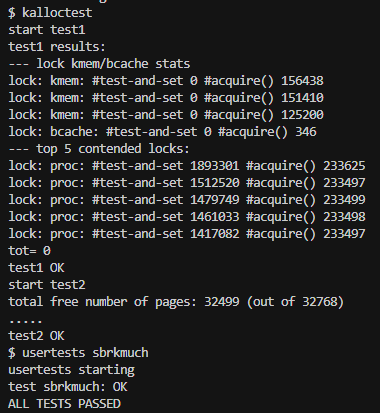
\includegraphics[width=0.4\textwidth]{test_memory_allocator_1}
	\caption{测试 memory allocater(1)}
	\label{fig:test_memory_allocator_1}
\end{figure}

\begin{figure}[!htb]
	\centering
	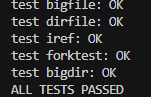
\includegraphics[width=0.5\textwidth]{test_memory_allocator_2}
	\caption{测试 memory allocater(2)}
	\label{fig:test_memory_allocator_2}
\end{figure}

\subsubsection{实现 buffer cache}

\begin{enumerate}
	\item 在 kernel/bio.c 中,根据提示,定义哈希桶结构,并在 \texttt{bcache} 中删除全局缓冲区链表,改为使用素数个散列桶,如\cref{lst:hashbuf} 所示。 
	\item 在 \texttt{binit} 中 
	\begin{enumerate*}
		\item 初始化散列桶的锁,
		\item 将所有散列桶的 \texttt{head->prev}、\texttt{head->next} 都指向自身表示为空,
		\item 将所有的缓冲区挂载到 \texttt{bucket[0]}桶上,
	\end{enumerate*}
	如\cref{lst:binit} 所示。
	\item 修改 \texttt{bpin} 和 \texttt{bunpin},使其修改的是对应序号桶的 \texttt{refcnt},如\cref{lst:bpin_and_bunpin} 所示。
	\item 在 kernel/buf.h 中添加新字段 \texttt{timestamp} ,使用时间戳作为 LRU 判定的法则。
	\item 修改 \texttt{brelse},不再获取全局锁,如\cref{lst:brelse} 所示。
	\item 修改 \texttt{bget},当没有找到指定的缓冲区时进行分配,分配方式是优先从当前列表遍历,找到一个没有引用且 \texttt{timestamp} 最小的缓冲区,如果没有就申请下一个桶的锁,并遍历该桶,找到后将该缓冲区从原来的桶移动到当前桶中,最多将所有桶都遍历完。在代码中要注意锁的释放。
	\item 完成修改后,运行 bcachetest 和 usertests 进行测试,测试通过,如\cref{lst:test_buffer_cache_1} 和 \cref{lst:test_buffer_cache_2} 所示。
\end{enumerate}

在 kernel/kalloc.c 中,将原先单个的 \texttt{kmem} 改为数量为 NCPU 的一组,对应修改 \texttt{kinit},如\cref{kmem_NCPU} 所示。 

\begin{listing}[!htb]
	\begin{minted}{c}
#define NBUCKET 13
#define HASH(number) (number % NBUCKET)

struct hashbuf{
    struct spinlock lock;
    struct buf head;
};

struct {
    struct hashbuf buckets[NBUCKET];
    struct buf buf[NBUF];
} bcache;
	\end{minted}
	\caption{修改 bcache 的结构}\label{lst:hashbuf}
\end{listing}

\begin{listing}[!htb]
	\begin{minted}{c}
void
binit(void)
{
    struct buf *b;

    for(int i = 0; i < NBUCKET; i++){
        initlock(&bcache.buckets[i].lock, "bcache");

        // Create linked list of buffers
        bcache.buckets[i].head.prev = &bcache.buckets[i].head;
        bcache.buckets[i].head.next = &bcache.buckets[i].head;
    }

    for(b = bcache.buf; b < bcache.buf+NBUF; b++){
        b->next = bcache.buckets[0].head.next;
        b->prev = &bcache.buckets[0].head;
        initsleeplock(&b->lock, "buffer");
        bcache.buckets[0].head.next->prev = b;
        bcache.buckets[0].head.next = b;
    }
}
	\end{minted}
	\caption{binit 函数的实现}\label{lst:bcache}
\end{listing}

\begin{listing}[!htb]
	\begin{minted}{c}
void
bpin(struct buf *b) {
    int bid = HASH(b->blockno);
    acquire(&bcache.buckets[bid].lock);
    b->refcnt++;
    release(&bcache.buckets[bid].lock);
}

void
bunpin(struct buf *b) {
    int bid = HASH(b->blockno);
    acquire(&bcache.buckets[bid].lock);
    b->refcnt--;
    release(&bcache.buckets[bid].lock);
}
	\end{minted}
	\caption{bpin 和 bunpin 的实现}\label{lst:bpin_and_bunpin}
\end{listing}

\begin{listing}[!htb]
	\begin{minted}{c}
void
brelse(struct buf *b)
{
    if(!holdingsleep(&b->lock))
    panic("brelse");

    int bid = HASH(b->blockno);

    releasesleep(&b->lock);
    
    acquire(&bcache.buckets[bid].lock);
    b->refcnt--;

    acquire(&tickslock);
    b->timestamp = ticks;
    release(&tickslock);

    release(&bcache.buckets[bid].lock);
}
	\end{minted}
	\caption{brelse 函数的实现}\label{lst:brelse}
\end{listing}

\begin{listing}[!htb]
	\begin{minted}[breaklines,breakanywhere,fontsize=\small]{c}
static struct buf* bget(uint dev, uint blockno) {
    struct buf *b;int bid = HASH(blockno);
    acquire(&bcache.buckets[bid].lock);
    // Is the block already cached?
    for(b = bcache.buckets[bid].head.next; b != &bcache.buckets[bid].head; b = b->next) {
        if(b->dev == dev && b->blockno == blockno) {
            b->refcnt++;
            acquire(&tickslock);
            b->timestamp = ticks;
            release(&tickslock);           
            release(&bcache.buckets[bid].lock);
            acquiresleep(&b->lock);
            return b;
        }
    }
    // Not cached.
    b = 0;
    struct buf *tmp;    
    for(int i = bid, cnt = 0; cnt < NBUCKET; i = (i+1)%NBUCKET, cnt++) {
        if(i != bid) {
            if(!holding(&bcache.buckets[i].lock))
            acquire(&bcache.buckets[i].lock);
            else continue;
        }          
        for(tmp = bcache.buckets[i].head.next; tmp != &bcache.buckets[bid].head; tmp = tmp->next)
        if(tmp->refcnt == 0 && (b == 0 || tmp->timestamp < b->timestamp))
        b = tmp;
        if(b) {
            if(i != bid) {
                release(&bcache.buckets[i].lock);
                // Remove and add to new bucket
                b->prev->next = b->next;
                b->next->prev = b->prev;
                b->next = bcache.buckets[bid].head.next;
                b->prev = &bcache.buckets[bid].head;
                bcache.buckets[bid].head.next->prev = b;
                bcache.buckets[bid].head.next = b;
            }           
            b->dev = dev;
            b->blockno = blockno;
            b->valid = 0;
            b->refcnt = 1;        
            acquire(&tickslock);
            b->timestamp = ticks;
            release(&tickslock);  
            release(&bcache.buckets[bid].lock);
            acquiresleep(&b->lock);
            return b;
        }
        else if(i != bid)
        release(&bcache.buckets[i].lock); 
    }
    panic("bget: no buffers");
}
	\end{minted}
	\caption{bget 函数的实现}\label{lst:bget}
\end{listing}

\begin{figure}[!htb]
	\centering
	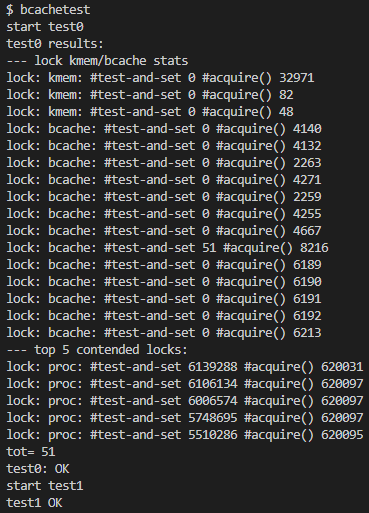
\includegraphics[width=0.4\textwidth]{test_buffer_cache_1}
	\caption{测试 buffer cache(1)}
	\label{fig:test_buffer_cache_1}
\end{figure}

\begin{figure}[!htb]
	\centering
	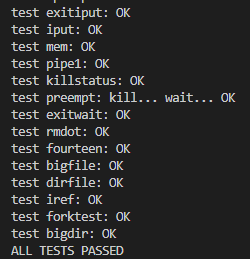
\includegraphics[width=0.3\textwidth]{test_buffer_cache_2}
	\caption{测试 buffer cache(2)}
	\label{fig:test_buffer_cache_2}
\end{figure}


\subsubsection{综合测试}

在 xv6-labs-2021 目录下创建一个 time.txt文件,记录该lab花费的时间。使用 \texttt{make grade} 对 lab8 进行综合测试,测试通过。

\begin{figure}[!htb]
	\centering
	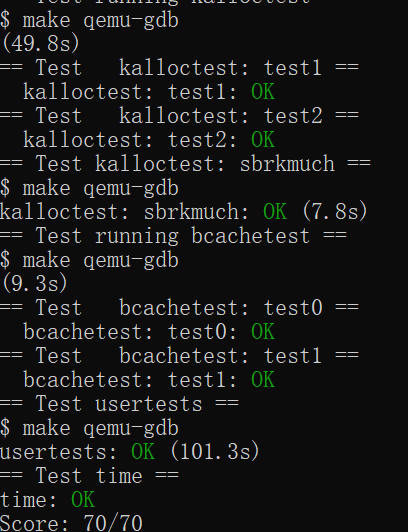
\includegraphics[width=0.35\textwidth]{test_lab8}
	\caption{测试 lab8}
	\label{fig:test_lab8}
\end{figure}

\subsection{实验小结}

实验 6 与本实验都是关于并行编程中问题的性能优化。用户可以实现用户级的多线程程序来更好地使用处理器资源,而分时系统通过多个进程的并发运行可以让多个程序看起来像同时在执行。在处理多线程或多进程中资源抢占而导致的锁竞争现象,常用的做法是通过分割资源并且分别加锁。锁的数量越多,单个锁上的冲突就越少(但是也要考虑锁的数量增多的负面影响)。 

我在两个实验中分别体会了控制进程的同步/互斥(实验 6)和分割资源来使锁竞争得到缓解、提高资源并行利用率。实验同时还涉及到了关中断、散列、资源分配等其他方面的细节,关联了我之前课程中学习的知识。从功能性角度来说,一个操作系统只需要拥有运行程序的能力,与用户交互的系统也最多需要增加并发运行这一个功能限制。而在实验中通过对资源的划分实现了提高系统效率和资源利用率这些非功能性需求,在一个面向现实世界的操作系统中,非功能性需求一样有重要地位。 

